\documentclass[hidelinks]{sig-alternate-05-2015}
\usepackage[utf8]{inputenc}
\usepackage{amsmath}
\usepackage[spanish]{babel}
\usepackage{float}
\usepackage{enumitem}
\usepackage{listings}
\usepackage{color}
\usepackage{hyperref}

\definecolor{dkgreen}{rgb}{0,0.6,0}
\definecolor{gray}{rgb}{0.5,0.5,0.5}
\definecolor{mauve}{rgb}{0.58,0,0.82}

\lstset{frame=tb,
  language=R,
  aboveskip=3mm,
  belowskip=3mm,
  showstringspaces=false,
  columns=flexible,
  basicstyle={\small\ttfamily},
  numbers=none,
  numberstyle=\tiny\color{blue},
  keywordstyle=\color{gray},
  commentstyle=\color{dkgreen},
  stringstyle=\color{mauve},
  breaklines=true,
  breakatwhitespace=true,
  tabsize=3
}

\setlist[enumerate]{label*=\arabic*.}
\pagenumbering{arabic}



\begin{document}
%%%%%%%%%%%%%%%%%%%%%%%%%%%%%%%%%%%%%%%%%%%
%% Título

\title{Clasificación sentimental de reseñas de libros en Goodreads como positivas o negativas usando técnicas de aprendizaje de máquinas
\subtitle{[Extended Abstract]
}}

%%%%%%%%%%%%%%%%%%%%%%%%%%%%%%%%%%%%%%%%%%%
%% Autores

\numberofauthors{2} 
\author{
% 1st. author
\alignauthor
Andrea Salcedo\\
       \affaddr{Universidad Simón Bolívar}\\
       \affaddr{Caracas, Venezuela}\\
       \email{andreacsalcedo@gmail.com}
% 2nd. author
\alignauthor
Reinaldo Verdugo\\
       \affaddr{Universidad Simón Bolívar}\\
       \affaddr{Caracas, Venezuela}\\
       \email{verdugoreinaldo@gmail.com}
}

\maketitle
\begin{abstract}

Goodreads es una red social que permite a sus usuarios calificar y recomendar libros gracias a un proceso de reseñas en el que los usuarios comentan sus experiencias al leer una determinada publicación y le asignan un valor entero entre 0 y 5. Con tan poca variedad de calificaciones, resulta conveniente revisar los comentarios escritos por los lectores para saber si esa reseña es positiva hacia la publicación o no, dependiendo del lenguaje y sentimientos que estén plasmados en la misma. 

Como el análisis de dichos sentimientos incluyen cierto componente subjetivo que dificulta la clasificación por parte de los humanos, nos damos a la tarea de utilizar algoritmos presentes en la inteligencia artificial que realicen dicho proceso y puedan etiquetar una reseña como positiva o negativa dependiendo del lenguaje incluido en la misma. Para ello, la métrica a utilizar consistirá en comparar la clasificación resultante con el valor numérico otorgado en la reseña (valores que serán tomados como positivos si son 4 o 5, negativos si son 1 y 2 o neutros si son iguales a 3). 

El aprendizaje será supervisado y usaremos reseñas calificadas como positivas o negativas para el entrenamiento. Se plantea la posibilidad de usar calificaciones neutrales para el conjunto de prueba. Además, se utilizarán los algoritmos de K-Nearest Neighbors, Support Vector Machines y Maximum Entropy para este aprendizaje y luego se hará una comparación de los resultados obtenidos.

Maximum Entropy obtuvo la mejor clasificación con un promedio del 82.60\% de datos clasificados correctamente comparado a K-Nearest Neighbors con uno del 67.75\% y a Support Vector Machines con uno del 77.65\%.

\end{abstract}

\keywords{Aprendizaje de máquinas, Goodreads, stemming, stopwords, reseñas, K-Nearest Neighbors (KNN), Support Vector Machines (SVM), Maximum Entropy Classifier (Maxent)}

%%%%%%%%%%%%%%%%%%%%%%%%%%%%%%%%%%%%%%%%
%% Planteamiento del problema
\section{Planteamiento del problema}
En este trabajo buscamos clasificar las reseñas de libros realizadas por usuarios de la comunidad de Goodreads \cite{chandler:goodreads}. Para dicha clasificación se tomarán en cuenta los sentimientos plasmados en la reseña, a fin de conocer si dicha crítica es positiva por contener sentimientos positivos (que hacen alusión a que el lector disfrutó de la lectura), o si por el contrario es negativa por contener sentimientos negativos (y por lo tanto mostrando descontento por parte del lector).
    
En muchas ocasiones a la hora de criticar un libro, surgen interrogantes como ¿qué número de estrellas debo otorgarle? o ¿dicho número de verdad refleja mi opinión respecto a la publicación? Además, existe la complicación adicional de que en Goodreads (red social centrada en la clasificación y recomendación de libros) \cite{chandler:goodreads} sólo se pueden colocar valores enteros entre 0 y 5; un libro que te parece lo bastante bueno como para tener más de 4 estrellas, pero no lo suficiente como para tener 5, torna complicado el proceso de calificación del mismo. 

Dichos contratiempos nos obligan a enfocarnos más en la reseña escrita que en la valoración para saber si un lector quedó contento con la lectura de algún libro, o no. Pero ¿qué tan precisos somos los humanos clasificando una reseña en base a las palabras que contiene? Creemos pertinente entonces utilizar algoritmos de clasificación ya presentes en la disciplina de la inteligencia artificial para desarrollar este proceso.

Para la clasificación de las reseñas se utilizó aprendizaje supervisado utilizando los algoritmos de K-Nearest Neighbors, Support Vector Machines y Maximum Entropy. Cada uno fue entrenado con el 70\% de los datos etiquetados como positivos o negativos dependiendo de la cantidad de estrellas otorgadas y se realizaron las pruebas con el 30\% restante. Se hicieron 30 experimentos por cada algoritmo y los resultados fueron promediados para luego ser comparados para obtener la mejor técnica de clasificación.

% Antecedentes
\subsection{Antecedentes}

Un análisis similar fue realizado con anterioridad en \textit{Thumbs up? Sentiment Classification using Machine Learning Techniques} de Bo Pang y Lillian Lee. En dicho trabajo realizaron un análisis de sentimientos para clasificar las reseñas de la base de datos de IMDB como positivas o negativas \cite{pang:thumbs up}.

Otros trabajos similares incluyen el de Karlgren y Cutting, en el que realizaron una investigación para determinar el género de los textos, los cuales podían incluir categorías subjetivas como 'editorial'.\cite{karlgren: text genres}

% Estructura
\subsection{Estructura del documento}

El presente documento se encuentra estructurado de la siguiente manera:
\begin{enumerate}

	\item Planteamiento del Problema
	\item Marco teórico
	\begin{enumerate}
		\item Conceptos
	\end{enumerate}
    \item Diseño de la Solución
    \begin{enumerate}
		\item Descripción del Clasificador
        \begin{enumerate}
            \item Algoritmos
		\end{enumerate}
	\end{enumerate}
    \item Implementación
    \begin{enumerate}
		\item Lenguajes y Plataformas de Desarrollo
		\item Obtención y Almacenamiento de Datos
        \item Preprocesamiento de los Datos
        \item Implementación de los Algoritmos
		\begin{enumerate}
			\item Preprocesamiento de Datos
			\item K-Nearest Neighbors
        	\item Support Vector Machines
            \item Maximum Entropy
	\end{enumerate}
	\end{enumerate}
    \item Resultados
    \begin{enumerate}
		\item Almacenamiento y Análisis de los Resultados
		\item Reseñas Neutras
        \item Limitaciones
	\end{enumerate}
    \item Conclusiones
    \item Referencias
    
\end{enumerate}
%%%%%%%%%%%%%%%%%%%%%%%%%%%%%%%%%%%%%%%%
%% Marco Teórico
\section{Marco teórico}

% Conceptos
\subsection{Conceptos}
\begin{itemize}

\item \textbf{Análisis de Sentimientos} se refiere al proceso por el que determinamos si una frase o acto de habla contiene una opinión, positiva o negativa, sobre una entidad concreta o sobre un concepto. Es un término que está muy ligado a las redes sociales pero que, en realidad, no está limitado a ellas.\cite{delgado:analisis}

\item \textbf{Goodreads} es el sitio para lectores y recomendaciones de libros más grande del mundo. Su misión es ayudar a sus usuarios a conseguir y compartir libros que amen.\cite{chandler:goodreads}

\item Una \textbf{reseña} es una evaluación o crítica constructiva, que puede ser positiva o negativa que depende de lo que el crítico analice, de objetos tales como una película, un videojuego, un anime, un libro, etc. El autor puede asignar al objeto criticado una calificación para indicar su mérito relativo con el objeto de aproximar a los lectores hacia lo descrito.\cite{wikipedia:review}

\item \textbf{Stemming} es un método para reducir una palabra a su raíz o a un stem o lema.\cite{wikipedia:stemming}.

Por ejemplo, las palabras \textit{like, liking, liked} pueden reducirse a su stem \textit{lik}.

\item \textbf{Stopwords} (en español, palabra vacía) es el nombre que reciben las palabras sin significado como artículos, pronombres, preposiciones, etc. que son filtradas antes o después del procesamiento de datos en lenguaje natural (texto).\cite{wikipedia:stopwords}

Por ejemplo: \textit{a, about, and, in, or}, etc.

\end{itemize}

%%%%%%%%%%%%%%%%%%%%%%%%%%%%%%%%%%%%%%%%
\section{Diseño de la solución}

%% Descripción del clasificador
\subsection{Descripción del Clasificador}

Se hizo uso de aprendizaje supervisado al contar con un conjunto de entrenamiento de reseñas clasificadas como positivas o negativas. Dicho conjunto consiste en el 70$\%$ de las reseñas conseguidas, quedando como conjunto de prueba el 30$\%$ restante. La tarea, métrica de perfomance y experiencia para este proyecto fueron los siguientes:

\begin{itemize}
\item \textbf{Tarea}: Clasificar reseñas de libros en Goodreads como positivas o negativas.

\item \textbf{Métrica de performance}: Comparar la clasificación con la calificación o el número de estrellas otorgadas de la reseña.

\item \textbf{Experiencia}: Reseñas obtenidas del API de Goodreads, etiquetadas como positivas, negativas o neutras utilizando el número de estrellas otorgadas. Es decir, una reseña negativa tiene 0, 1 o 2 estrellas, una neutra tiene 3 y una positiva tiene 4 o 5. Sólo se tomarán en cuenta las reseñas positivas y negativas para el entrenamiento.

\end{itemize}

% Algoritmos
\subsubsection{Algoritmos}

Para el análisis de texto se utilizaron tres algoritmos, cada uno ofreciendo un enfoque distinto para atacar el problema:

\begin{enumerate}

\item \textbf{Algoritmo K-Nearest Neighbor (KNN)} o \textbf{K-Vecinos más cercanos}. Basado en el método \textit{k}-nn de Fix y Hodges en 1951\cite{fix:knn} es una forma de aprendizaje supervisada basada en la clasificación no paramétrica de objetos, realizando un entrenamiento mediante ejemplos cercanos en el espacio de los elementos. 

\vskip -5pt
%% Figure 1 
\begin{figure}[H]
\centering
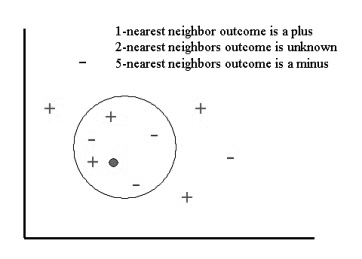
\includegraphics[keepaspectratio=true,scale=0.75]{knn.jpg}
\vskip -6pt
\caption{Representación del valor resultante de aplicar algoritmo KNN para tres valores de K: 1, 2 y 5 \cite{statsoft:knn}}
\end{figure}
\vskip -5pt

En nuestro caso, aplicamos dicho método de reconocimiento a la clasificación de textos donde los ejemplos (o vecinos) cercanos corresponden a los textos con la mayor cantidad de palabras similares (tomando en cuenta el uso de stemming).

Por ejemplo, para la reseña:
\vskip 3pt
\textit{"It's rather \textbf{like} a lifetime special-- \textbf{pleasant}, sweet, and forgettable"} 
\vskip 3pt

puede considerarse como vecina cercana la reseña:

\vskip 3pt
\textit{"I \textbf{liked} this book, made for a \textbf{pleasant} evening"} 
\vskip 3pt

debido a los dos stems que coinciden. 

\item \textbf{Support Vector Machines (SVM)} o \textbf{Máquina de Vectores de Soporte} se centra en dividir los datos (en este caso reseñas) en dos clases: la clase de reseñas positivas, y la clase de reseñas negativas. Entre ambas clases se busca un \textbf{vector frontera o vector de pesos} \begin{math}\vec{\textbf{w}}\end{math} que debe cumplir con las siguientes condiciones:

\begin{itemize}

\item \begin{displaymath}\sum_{i} w_{i} d_{i,j} \geqslant 1 \end{displaymath} todas las reseñas positivas que tienen una calificación $\geqslant$ 1

\item \begin{displaymath}\sum_{i} w_{i} d_{i,j} \leq -1 \end{displaymath} todas las reseñas negativas que tienen una calificación $\leq$ -1

\item \begin{displaymath} min\lVert \mathbf{\vec{w}} \rVert\end{displaymath} se debe maximizar el espacio entre las fronteras minimizando el tamaño del vector \begin{math}\vec{w}\end{math}
\end{itemize}

Como en la mayoría de las implementaciones, en esta solución el vector frontera consiste en la suma de las reseñas positivas multiplicadas por un peso particular menos la suma de las reseñas negativas, también multiplicadas por un peso particular, como se muestra a continuación:

\begin{displaymath} \vec{w} = \sum_{j \in +} \alpha_{j} \vec{d}_{j} - \sum_{j \in -} \alpha_{j} \vec{d}_{j}  \end{displaymath}

donde $\alpha$ corresponde al peso particular para cada reseña. Para este experimento, se utilizará $\alpha$ = 2 (Ver capítulo 4. Implementación)

\vskip -5pt
%% Figure 2 
\begin{figure}[H]
\centering
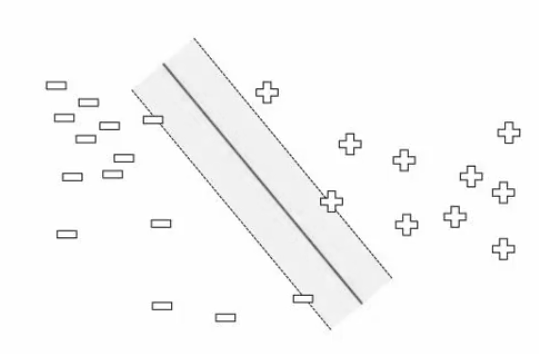
\includegraphics[keepaspectratio=true,scale=0.42]{svm_example_lavrenko.png}
\caption{Representación de las dos clases separadas por el vector frontera \cite{lavrenko:svm}}
\end{figure}

\item \textbf{Maximum Entropy}. También conocido como \textbf{Multinomial logistic regression} es una solución particular del problema de clasificación que asume que una combinación lineal de los \textbf{rasgos} (o características) observados y algunos parámetros específicos del problema pueden usarse para determinar la probabilidad de cada valor venidero de la variable dependiente \cite{wikipedia:maxent}, que este caso sería si una reseña es positiva o negativa.

Para nuestro problema en particular, aplicamos Maxent en el procesamiento del lenguaje natural. En esta aplicación cada rasgo particular que distingue los datos son por supuesto, las palabras. Cada palabra se codifica como un \textit{String} para poder utilizarse en una tabla de Hash. Para cada rasgo se construye una función que incluye a dicho rasgo con su respectiva clase, y un valor de peso. 
 
El propósito del algoritmo de Maxent es maximizar la entropía, la cual es la incertidumbre de la distribución. Para esto se necesita calcular para cada evento considerado en la distribución los siguientes datos:

Dado un evento \textit{x} se tiene la probabilidad de que el evento \textit{x} ocurra: \begin{displaymath}p_x\end{displaymath} y la "sorpresa", o la incertidumbre de que ocurra el evento \textit{x}: \begin{displaymath}log(1/p_x)\end{displaymath}

Si la probabilidad del evento \textit{x} es alta, entonces la sorpresa del mismo sería baja, ya que es más esperado que ocurra que no. 

Entonces para calcular la entropía de una probabilidad, se calcula la sorpresa esperada del evento \textit{x}:\begin{displaymath}H(p) = E_{p}[log_2(1/p_x)] = -\sum_{x} p_{x} log_2(p_{x}) \end{displaymath} y se consideran todas las restricciones adicionales de los rasgos. 
En el caso de este proyecto, las restricciones serían que la sorpresa esperada de cada palabra sea lo más cercana a la ocurrencia verdadera de la misma \cite{jurafsky:maxent}. 

Maxent sirve como alternativa a los clasificadores de Naive Bayes porque no asumen dependencia para cada característica o rasgo. A pesar de que Maxent no es recomendado por su lentitud y porque no es óptimo cuando debe aprender muchas clases, para nuestro problema en particular donde sólo entrenamos con dos, no presenta tantos inconvenientes. 

\end{enumerate}

%%%%%%%%%%%%%%%%%%%%%%%%%%%%%%%%%%%%%%%%
\section{Implementación}

\subsection{Lenguajes y Plataformas de Desarrollo}

Para el desarrollo del proyecto se utilizaron dos lenguajes de programación:

\begin{itemize}
	\item \textbf{Python} - versión \textbf{2.7.10}. El cual sirvió para obtener, preprocesar y almacenar los datos necesarios para el proyecto. Se escogió Python por la facilidad que presenta en la lectura de archivos y el manejo de Strings y listas, fundamentales para los pasos mencionados anteriormente.
    
    Con este lenguaje se incluyeron las librerías \textbf{Requests} y \textbf{ElementTree XML} para realizar solicitudes HTTP y parsear documentos XML, respectivamente.
    
    \item \textbf{R} - versión \textbf{3.2.4}. Con el cual se realizó la implementación de los tres algoritmos. Se escogió R debido a su eficacia con el procesamiento de datos y su eficiencia con métodos estadísticos. 
    
    Mediante este lenguaje se utilizaron las librerías \textbf{tm}, \textbf{plyr}, \textbf{class}, \textbf{e1071} y \textbf{maxent} en la implementación de los algoritmos (Ver 4.4).
   
    
\end{itemize}

\subsection{Obtención y Almacenamiento de Datos}
Mediante el uso de Python, logramos obtener los datos proporcionados por el API de Goodreads. Para esto, se utilizó la librería \textbf{Requests} para realizar solicitudes HTTP para obtener las reseñas. Se realizaron dos tipos de solicitudes al API, uno para obtener la reseñas más recientes (cada solicitud devuelve las 20 más recientes) y otro para obtener una reseña en específico. Se aplicó el segundo para tener más reseñas negativas, ya que el sistema arrojó más reseñas positivas.

Luego, las reseñas más recientes se almacenaron en su estructura original en archivos XML con la estampilla de tiempo correspondiente en la carpeta \texttt{/data/original}. Las reseñas individuales también fueron guardadas en su estructura original XML pero en la carpeta \texttt{/data/individual} con el id de la misma.

Para facilitar el proceso de aprendizaje, se realizó una limpieza manual de los datos obtenidos de la siguiente manera:
\begin{itemize}
\item Se eliminaron reseñas donde sólo estaba la calificación pero ninguna opinión fue otorgada.
\item Se borraron las reseñas que estaban en otros idiomas, ya que el API no provee información sobre el idioma de la reseña.
\item Se eliminaron reseñas que eran positivas pero tenían una calificación de 0.
\item Se borraron las reseñas que sólo tenían un resumen del libro, ya que este tipo de reseña no expresa ninguna opinión o sentimiento.
\end{itemize}

Después de almacenar y limpiar manualmente todos los datos necesarios, se leyeron todos los archivos XML y se procesan para obtener una lista de \textit{Reviews}, un objeto que representa una reseña con la siguiente información: el id, la calificación y el texto de la reseña. Posteriormente, esta lista se utilizó para separar y guardar cada tipo de reseña (positiva, neutra y negativa) en su archivo respectivo. Estas reseñas pueden encontrarse en el directorio \texttt{/data/divided}.

La clase neutra sólo se utilizará para probar cómo se clasifican las reseñas, ya que algunas reseñas neutras tienden a ser más positivas y otras más negativas.

\subsection{Preprocesamiento de los Datos}

Después de separar cada reseña en su clase respectiva, se realizó un preprocesamiento de las mismas. Este preprocesamiento incluyó: 
\begin{itemize}
\item Se eliminaron las etiquetas de HTML.
\item Se eliminó la puntuación.
\item Se quitaron los números.
\item Se realizó el proceso de Stemming para condensar en un stem los términos de la misma raíz.
\item Eliminación de palabras sin significado (stopwords).
\item Todo el texto de la reseña se convirtió a minúscula. 
\item Se borraron los espacios en blanco.
\end{itemize}

\subsection{Implementación de los Algoritmos}

\subsubsection{Preprocesamiento de Datos}
Para el preprocesamiento general de los datos se utilizó la librería \texttt{tm}. Con esta librería se creó un objeto llamado \textit{Corpus} para la representación de una colección de textos. Luego, este objeto fue manipulado para eliminar puntuación, números, stopwords y espacios vacíos; hacer stemming y transformar los textos a minúscula. Luego los datos preprocesados fueron guardados en archivos \texttt{.csv} para luego ser utilizados en los tres distintos algoritmos.   

\subsubsection{K-Nearest Neighbors}
Para el algoritmo de K-Nearest Neighbors se utilizaron las librerías \texttt{plyr} y \texttt{class}. La primera para poder combinar los conjuntos de datos de las reseñas positivas y negativas y la segunda para la utilización del algoritmo ya implementado de KNN.

\lstset{language=R}
\begin{lstlisting}
classifyKnn <- knn(reviewsWithoutTarget[trainSet,], reviewsWithoutTarget[testSet,], reviewsClass[trainSet])
\end{lstlisting}

\subsubsection{Support Vector Machines}
Para el algoritmo Support Vector Machines se utilizó la librería \texttt{e1071}. De esta librería se utilizaron las funciones \textit{svm} para el entrenamiento y \textit{predict} para clasificar el conjunto de prueba utilizando el modelo de SVM obtenido de la primera.

\lstset{language=R}
\begin{lstlisting}
svmModel <- svm(class ~ ., data = trainSet, gamma = 0.75, cost = 2)
prediction <- predict(svmModel, testSet[-2])
\end{lstlisting}

\subsubsection{Maximum Entropy}
Para el algoritmo Maximum Entropy se utilizó la librería \texttt{maxent}. Para el entrenamiento de Maxent, se utilizó la función \textit{maxent} que devolvió un modelo que luego fue utilizado en la función \textit{predict} para clasificar el conjunto de prueba.

\lstset{language=R}
\begin{lstlisting}
model <- maxent(trainSet,trainSetClass)
classifiedTestSet <- predict(model,testSet)
\end{lstlisting}

%%%%%%%%%%%%%%%%%%%%%%%%%%%%%%%%%%%%%%%%%%%%%%%%%%%%%%%%%%%
\section{Experimentos y Resultados}

\subsection{Almacenamiento y Análisis de los Resultados}

Para nuestro experimento logramos contar con un total de 1782 reseñas, distribuidas de la siguiente manera:
\begin{itemize}

\item 1154 positivas (rating de 4 o 5)
\item 350 negativas (rating de 0, 1 o 2 )
\item 278 neutras (rating de 3, utilizadas en la sección 5.2)

\end{itemize}
Una corrida de cualquiera de los tres algoritmos incluye el entrenamiento con el 70\% de los datos y la clasificación con el 30\% restante. Además, se devuelve la matriz de confusión de los resultados y el tamaño del conjunto de prueba. Estos datos son luego almacenados en un archivo \texttt{.RData} en el directorio \texttt{/results/}. 

Para cada algoritmo, debido a sus naturalezas estocásticas, se realizaron 30 corridas para luego analizarlas en el archivo \texttt{averages.r} y obtener un promedio de la exactitud, precisión, sensibilidad, especificidad y error del algoritmo.

En las tablas \ref{table:MC-KNN}, \ref{table:MC-SVM} y \ref{table:MC-MAXENT} se muestran las matrices de confusión del mejor resultado de cada algoritmo y en las tablas \ref{table:KNN}, \ref{table:SVM} y \ref{table:MAXENT} se muestran las medidas de exactitud, precisión, sensibilidad, especificidad y error calculadas a partir de las matrices.

\begin{table}[H]
\centering
\caption{Matriz de Confusión del Mejor Resultado de KNN}
\begin{tabular}{|c|c|c|} 					\hline
Predicción / Real	& Positiva 	& Negativa 	\\ \hline
Positiva 			& 308 		& 67 		\\ \hline
Negativa 			& 38 		& 38		\\
\hline\end{tabular}
\label{table:MC-KNN}
\end{table}

\begin{table}[H]
\centering
\caption{Mejor Resultado de KNN}
\begin{tabular}{|c|c|} 			\hline
Medida  		& Porcentaje 	\\ \hline
Exactitud 		& 76.72			\\ \hline
Precisión 		& 82.13			\\ \hline
Sensibilidad 	& 89.02			\\ \hline
Especificidad	& 36.19			\\ \hline
Error			& 23.28 		\\
\hline\end{tabular}
\label{table:KNN}
\end{table}

Podemos observar que el algoritmo KNN se desempeñó medianamente bien, generando una tasa de error de 23.28$\%$ de los datos.

Dicho error es causado principalmente por las reseñas negativas. En la matriz de confusión se puede apreciar que 67 reseñas negativas fueron clasificadas como positivas. 

\begin{table}[H]
\centering
\caption{Matriz de Confusión del Mejor Resultado de SVM}
\begin{tabular}{|c|c|c|} 					\hline
Predicción / Real	& Positiva 	& Negativa 	\\ \hline
Positiva 			& 329 		& 93 		\\ \hline
Negativa 			& 0 		& 7			\\
\hline\end{tabular}
\label{table:MC-SVM}
\end{table}

\begin{table}[H]
\centering
\caption{Mejor Resultado de SVM}
\begin{tabular}{|c|c|} 			\hline
Medida  		& Porcentaje 	\\ \hline
Exactitud 		& 78.32			\\ \hline
Precisión 		& 77.96			\\ \hline
Sensibilidad 	& 100			\\ \hline
Especificidad	& 7				\\ \hline
Error			& 21.68 		\\
\hline\end{tabular}
\label{table:SVM}
\end{table}

En el caso de SVM, los resultados presentan una mejoría ambigua: aunque el error se redujo de 23.28$\%$ a 21.68$\%$, las clasificaciones no son mejores. Como se puede observar en la tabla \ref{table:MC-SVM}, la clasificación de negativas empeora al clasificar 93 de ellas como positivas. Dichos resultados disminuyen medidas como la precisión, y drásticamente la especificidad (Ver tabla \ref{table:SVM}).

\begin{table}[H]
\centering
\caption{Matriz de Confusión del Mejor Resultado de MAXENT}
\begin{tabular}{|c|c|c|} 					\hline
Predicción / Real	& Positiva 	& Negativa 	\\ \hline
Positiva 			& 311 		& 31 		\\ \hline
Negativa 			& 35 		& 74		\\
\hline\end{tabular}
\label{table:MC-MAXENT}
\end{table}


\begin{table}[H]
\centering
\caption{Mejor Resultado de MAXENT}
\begin{tabular}{|c|c|} 			\hline
Medida  		& Porcentaje 	\\ \hline
Exactitud 		& 85.37			\\ \hline
Precisión 		& 90.94			\\ \hline
Sensibilidad 	& 89.88			\\ \hline
Especificidad	& 70.48			\\ \hline
Error			& 14.63 		\\
\hline\end{tabular}
\label{table:MAXENT}
\end{table}

Con Maxent los resultados fueron mucho más alentadores. El error logró reducirse a 14.63$\%$ generando una exactitud y una precisión de 85.37$\%$ y 90.94$\%$, respectivamente.

\vspace*{1\baselineskip}

\begin{table*}
\centering
\caption{Promedio de los resultados de cada algoritmo (30 corridas)}
\begin{tabular}{|c|c|c|c|} 								\hline
Medida  		& KNN (\%)	& SVM (\%)	& MAXENT (\%)	\\ \hline
Exactitud 		& 67.75		& 77.65		& \textbf{82.60} \\ \hline
Precisión 		& 84.98 	& 77.45 	& \textbf{89.50}			\\ \hline
Sensibilidad 	& 70.39 	& 99.97 	& \textbf{88.04}			\\ \hline
Especificidad	& 59.02 	& 04.23 	& \textbf{63.29}			\\ \hline
Error			& 32.25		& 22.35		& \textbf{17.40}			\\
\hline\end{tabular}
\label{table:RESULTS}
\end{table*}

Comparando entre los clasificadores de KNN y SVM en la tabla \ref{table:RESULTS} en la página \pageref{table:RESULTS}, SVM obtuvo una mejor clasificación en cuanto la precisión y el tamaño del error. Sin embargo, la precisión (detección correcta de la clase positiva) y especificidad (detección correcta de la clase negativa) fueron mayores en el clasificador KNN. Como muestra la tabla, SVM no logra clasificar bien las reseñas negativas, dado que su valor de la especificidad es muy bajo (en sólo 4\%).  

Este resultado puede ser debido a cómo funciona el algoritmo de KNN y su uso de palabras y frases comunes entre datos para la clasificación de los mismos. Durante la limpieza de los datos, se notó que las reseñas tienden a utilizar palabras y frases similares, como: \textit{"wonderful"}, \textit{$"$amazing"}, \textit{"great book"}, \textit{"must read"} y \textit{"wow"} para las positivas y \textit{"meh"}, \textit{"terrible"}, \textit{"disappointing"} y \textit{"horrible"} para las negativas. Por lo tanto, como hay tantas palabras y frases reutilizadas, el algoritmo KNN pudo detectar mejor entre las clases positivas y negativas que el SVM. 

El mejor clasificador fue el de Maximum Entropy, que logró clasificar correctamente en promedio el 82.60\% de los datos de prueba. En la tabla \ref{table:MAXENT} se muestra el mejor clasificador de éste, que clasificó correctamente el 85.37\% de los datos del conjunto de prueba. Este conjunto estaba compuesto de 346 reseñas positivas y 105 negativas, con un total de 451 reseñas, como muestra la tabla \ref{table:MC-MAXENT}. El error fue de un 14.63\%.

Es importante destacar que en el algoritmo de Maxent las palabras son independientes. Por ejemplo, \textit{"must read"} es una frase que aparece constantemente pero la palabra \textit{"must"} y la palabra \textit{"read"} son consideradas aparte, el caso contrario del algoritmo KNN. Además, el algoritmo sólo considera si la palabra aparece al menos una vez en el texto. Es decir, la aparición y no la repetición de una palabra es lo que afecta la clasificación de la reseña. 

\subsection{Reseñas Neutras}

Luego de conseguir el algoritmo que arrojaba los mejores resultados para nuestro problema, nos pareció un experimento interesante intentar clasificar las reseñas neutras en positivas o negativas.

Utilizamos de nuevo \textbf{Maxent} para entrenar con todos los ejemplos de reseñas (1502 en total) y se usaron las 278 neutras para el conjunto de prueba. La mayoría resultaron ser clasificadas como positivas. Los resultados pueden consultarse en la siguiente tabla \ref{table:NEUTRAL}.

\begin{table}[H]
\centering
\caption{Clasificación de reseñas neutras en positivas o negativas con MAXENT}
\begin{tabular}{|c|c|} 	\hline
Positiva 	& Negativa 	\\ \hline
257 		& 21 		\\
\hline\end{tabular}
\label{table:NEUTRAL}
\end{table}

Para analizar el por qué de estos resultados, observamos las reseñas neutras y nos percatamos de que muchas de ellas presentaban términos como \textit{``cute"} o \textit{``I liked the book, but not enough to..."} los que podrían haber hecho pensar al clasificador que las mismas eran positivas.

\subsection{Limitaciones}

Durante los experimentos de este proyecto, hubo varias limitaciones que afectaron los resultados.
\begin{itemize}
\item El API de Goodreads sólo devuelve las 20 reseñas más recientes y esta solicitud se actualiza cada 10 minutos. Es decir, si una solicitud se realiza a las 10:30 a.m y otra a las 10:35 a.m, ambas devolverán las mismas reseñas. Por lo tanto se debe esperar al menos 10 minutos para obtener nuevos datos.
\item Durante la obtención de los datos, se logró obtener más reseñas positivas que negativas. Por lo tanto, se tuvo que buscar reseñas negativas manualmente para tener un conjunto de datos más balanceado. Esto tomó mucho más tiempo de lo esperado e igualmente no se consiguió el tiempo para balancear completamente los datos. Esta diferencia en la cantidad de reseñas positivas y reseñas negativas afectó los resultados de este proyecto.
\item Un problema general del análisis de sentimiento es la detección de sarcasmo y el uso de referencias culturales, referencias a otros libros, modismos y emoticonos. La consideración de estos elementos sería una posible mejora a este proyecto.
\end{itemize}
\vspace*{1\baselineskip}

%%%%%%%%%%%%%%%%%%%%%%%%%%%%%%%%%%%%%%%%%%%%%%%%%%%%%%%%
\section{Conclusiones}
En este proyecto se deseaba poder clasificar reseñas realizadas por los usuarios de la comunidad de Goodreads en reseñas positivas y negativas, ya que no siempre es fácil saber si el número de estrellas otorgadas refleja correctamente la opinión plasmada por el usuario en una reseña.

Para esto se utilizó el aprendizaje supervisado donde la tarea consistió en clasificar las reseñas como positivas o negativas, la métrica utilizada fue comparar la clasificación con el número de estrellas de la reseña y finalmente la experiencia presente fueron las reseñas etiquetadas como positivas o negativas dependiendo del número de estrellas otorgadas por el usuario. 

Los algoritmos utilizados para el aprendizaje supervisado fueron principalemente: K-Nearest Neighbor, Support Vector Machine y Maximum Entropy Classifier, cada uno brindando un enfoque distinto que luego fue comparado a través de los resultados. Para cada algoritmo se realizaron 30 experimentos para obtener un mejor promedio de la exactitud, la precisión, la sensibilidad, la especificidad y el error. El mejor clasificador fue el de Maxent, que logró clasificar correctamente en promedio el 82.60\% de los datos de prueba.

Según los resultados obtenidos, pareciera ser justo asumir que muchas de las reseñas que son calificadas con muy pocas estrellas (negativas), incluyen un lenguaje que no pareciera reflejar dicho descontento. Es evidente entonces, como pensábamos al inicio del proyecto, que no todas las reseñas con el mismo número de estrellas son iguales, y que dentro de ellas existen matices que expresan mejores o peores sentimientos con respecto a las lecturas.

Finalmente, para futuros trabajos sería conveniente experimentar con una cantidad mayor de reseñas positivas y negativas, para ver si esto afecta considerablemente (o no) el resultado de cada algoritmo utilizado. Además, otro problema interesante a considerar sería la inclusión de la clase neutra durante el entrenamiento y examinar qué tanto ésta puede influir en la etapa de clasificación.

\vspace*{1\baselineskip}
%\end{document}  % This is where a 'short' article might terminate

%%%%%%%%%%%%%%%%%%%%%%%%%%%%%%%%%%%%%%%%
%% BIBLIOGRAPHY
\begin{thebibliography}{1}
\bibliographystyle{unsrt}

% HAY QUE ARREGLAR ESTAS REFERENCIAS COMO DEBEN SER

\bibitem{chandler:goodreads} Chandler, O. \emph{About Goodreads}, disponible en \url{https://www.goodreads.com/about/us}. Revisado por última vez el 26 de marzo de 2016 en navegador Mozilla Firefox.

\bibitem{dataschool:confusionMatrix} Data School. \emph{Simple guide to confusion matrix terminology},  disponible en
\url{http://www.dataschool.io/simple-guide-to-confusion-matrix-terminology/} Revisado por última vez el 27 de marzo de 2016 en navegador Mozilla Firefox.

\bibitem{delgado:analisis} Delgado Tenorio, M. \emph{¿Qué es el análisis del sentimiento?},  disponible en \url{http://manueldelgado.com/que-es-el-analisis-del-sentimiento/}. Revisado por última vez el 25 de marzo de 2016 en navegador Mozilla Firefox.

\bibitem{fix:knn} Fix, E. and Hodges, J.L (1989). \emph{ An Important Contribution to Nonparametric Discriminant Analysis and Density Estimation: Commentary on Fix and Hodges }, International Statistical Review / Revue Internationale de Statistique 57 (3): 233–238, 1951.

\bibitem{jurafsky:maxent} Jurafsky, D. and Manning, C. \emph{The Maximum Entropy Model Presentation}, disponible en \url{https://www.youtube.com/watch?v=Qn4vZvOEqB0}

\bibitem{jurafsky:intro} Jurafsky, D. and Manning, C. \emph{Course Introduction - Stanford NLP}, disponible en \url{https://www.youtube.com/watch?v=nfoudtpBV68&list=PL6397E4B26D00A269}

\bibitem{jurafsky:building a maxent} Jurafsky, D. and  Manning, C. \emph{Building a Maxent Model The Nuts and Bolts}, disponible en  \url{https://www.youtube.com/watch?v=mgBPp2h8qm8\&list=PL6397E4B26D00A269\&index=41\&spfreload=10}

\bibitem{karlgren: text genres} Karlgren, J. and Cutting, D. \emph{Recog- nizing text genres with simple metrics using dis- criminant analysis}. In Proc. of COLING. 1994. 

\bibitem{lavrenko:svm} Lavrenko, V. \emph{Text classification 4: Support Vector Machine}, disponible en \url{www.youtube.com/watch?v=A7FeQekjd9Q} Revisado por última vez el 26 de marzo de 2016 en navegador Mozilla Firefox.

\bibitem{pang:thumbs up} Pang, B., Lee, L. and Vaithyanathan, S. \emph{Thumbs up?: sentiment classification using machine learning techniques}, Proceedings of the ACL-02 conference on Empirical methods in natural language processing-Volume 10. Association for Computational Linguistics, 2002.

\bibitem{statsoft:knn}  Statsoft. \emph{k-Nearest Neighbors}, disponible en \url{http://www.statsoft.com/textbook/k-nearest-neighbors}. Revisado por última vez el 26 de marzo de 2016 en navegador Mozilla Firefox.

\bibitem{wikipedia:k-neighbors} Wikipedia. \emph{K-vecinos más cercanos}, disponible en \url{http://es.wikipedia.org/wiki/K-vecinos\_más\_cercanos}. Revisado por última vez el 26 de marzo de 2016 en navegador Mozilla Firefox.

\bibitem{wikipedia:stopwords} Wikipedia. \emph{Palabra vacía"}, disponible en \url{https://es.wikipedia.org/wiki/Palabra_vacía}. Revisado por última vez el 26 de marzo de 2016 en navegador Mozilla Firefox.

\bibitem{wikipedia:maxent} Wikipedia. \emph{Regresión logística multinomial}, disponible en \url{https://es.wikipedia.org/wiki/Regresi\%C3\%B3n_log\%C3\%ADstica_multinomial}. Revisado por última vez el 28 de marzo de 2016 en navegador Mozilla Firefox.

\bibitem{wikipedia:review} Wikipedia. \emph{Reseña}, disponible en \url{https://es.wikipedia.org/wiki/Rese\%C3\%B1a}. Revisado por última vez el 26 de marzo de 2016 en navegador Mozilla Firefox.

\bibitem{wikipedia:stemming} Wikipedia. \emph{Stemming}, disponible en \url{https://es.wikipedia.org/wiki/Stemming}. Revisado por última vez el 26 de marzo de 2016 en navegador Mozilla Firefox.



\end{thebibliography}esto 
\end{document}
